\chapter{Real-time application development} 

\label{Chapter6} 

\lhead{Chapter 6. \emph{Real-time application development}} 

The real-time application is based on a two-tier architecture, organized as follows:
\begin{itemize}
\item the server machine runs a Python Flask application, and it is responsible for generating playlists and audio
\item the client displays an HTML web-page that collects user interactions and sends them to the server machine for realtime editing of playlists. Additionally, it receives audio streaming from the server.
\end{itemize}

Therefore, the realtime computation of music similarity happens on the server machine.

\section{The server application}
\label{sec:rtserver}
As already stated above, the server application is in charge of offering several features: it generates the playlist, sending audio and additional information to the client (such as \textit{artist} and \textit{title} of current playing piece, so that the client can display them for the user on the GUI). Additionally it has to generate audio, that will be streamed to the client in order for the user to listen to it through its own device. For generating the playlist, a realtime music similarity algorithm with very good performance must run on the server. \\ Many Python web frameworks are available; the most used ones are Django\footnote{\url{https://www.djangoproject.com/}}, Flask\footnote{\url{http://flask.pocoo.org/}} and Pyramid\footnote{\url{http://www.pylonsproject.org/}}. This realtime server application has been based upon Flask framework, that is a lightweight web application framework written in Python and based on the WSGI toolkit\footnote{A specification for universal communication between web servers and web applications or frameworks for Python programming language. Published on December 2003 by its author Phillip J. Eby, it has become a standard for Python web application development.} and Jinja2 template engine\footnote{\url{http://jinja.pocoo.org/docs/dev/}}. It is provided with a BSD license and, contrarily to Django and Pyramid, is aimed at small applications with simple requirements. Its first version was released in 2010 and it comes with a great usability, where a simple \textit{``Hello World''} web-app can be written with only 7 lines of source code\footnote{\url{http://flask.pocoo.org/docs/0.10/quickstart/#a-minimal-application}}. Web application framework are usually thought to be separated into several conceptual units called ``apps'', each one providing different functionalities to the system. Flask is intended to make really simple the development of a single app; many others may be added, but in this latter case Django and Pyramid may provide a better ease of use. \\ All of these factors have lead to the choice of this framework for our system: the web platform to develop is actually intended to be quite simple, displaying just the main GUI and a few more details and options for the user. Given that the application is meant to be offered just to one client at time, we decided to use the builtin server of Flask also on production; indeed, we considered a full deployment option (such as Apache or CGI) to be a waste of resources for this simple use case. The server application executes two parallel tasks: the generation of the playlist, based on realtime computation of music similarity, and the generation and streaming of this playlist to the client of the audio. It furthermore provides several methods that are handled by Flask routing techniques and invoked at specific interaction of the user with the client application; these methods have deep impact on the generation of the playlist and allow the user real-time control over this process. 

\begin{figure}
\begin{center}

\includegraphics[scale=0.75]{Figures/flask.png}
    \rule{25em}{0.5pt}
  \caption[Flask]{Flask logo.}
  \label{fig:Flask}
\end{center}
\end{figure}

\subsection{Realtime computation of music similarity and playlist generation}
\label{subsec:rtalgorithm}
As we mentioned, this computation is performed on the server machine, for the hardware configuration of the interactive kiosk has been unknown until the beginning of the exhibition, and might have not been able to achieve good performance with the software developed. The hardware configuration of the server machine is shown in table~\ref{table:serverhardware}. 

\begin{center}
\begin{longtable}{ p{.25\textwidth}  p{.45\textwidth} } 
\toprule
\textbf{CPU}   & Intel\textregistered  Core\texttrademark 2 Quad Processor Q6600 @ 2.40GHz \\ \midrule
\textbf{RAM}   & 2GB DDR2 @ 800MHz  \\ \midrule
\textbf{Hard Disk Drive} & 5400rpm \\ \midrule
\textbf{OS} & Linux Mint 17.1 ``Rebecca'' (32bit) \\ \bottomrule
\caption[Hardware configuration of the server machine]{Hardware configuration of the server machine.}
\label{table:serverhardware}
\end{longtable}
\end{center}

The task for generating the playlist follows a well-defined schema: at first, the FastMap computed as described in section~\ref{sec:fastmap} is loaded into memory; this process usually takes just few seconds. A random point of this map is pick, and will be used as the first excerpt of the playlist. This excerpt in then put inside the playlist, a Python dictionary whose keys are the position of the elements inside the playlist and the corresponding values are tuples containing several important aspects for the playback; the details of these tuples are shown in table~\ref{table:playlistelements}.

\begin{center}
\begin{longtable}{| p{.12\textwidth} | p{.12\textwidth} | p{.12\textwidth} | p{.12\textwidth} | p{.12\textwidth} | p{.12\textwidth} |} 
\hline
URI of file & Song title & Song artist & Song Year & Starting time & Ending Time \\ \hline
\caption[Element of playlist]{Information stored for each element of the playlist.}
\label{table:playlistelements}
\end{longtable}
\end{center}

Once the first segment is picked, the application enters in a loop in which each iteration ends in adding a new excerpt to the playlist. The comparison of music similarity is always performed between all the candidate elements of the FastMap and the last element of the playlist. The procedure invoked in this loop can be summarized as follows:
\begin{enumerate}
\item If any user interaction with sliders or knobs has happened since the last iteration, delete the content of playlist. This allows users to immediately hear musical differences in the playlist as soon as they interact with the client application. 
\item Delete already played elements from the playlist in order to avoid memory leaks
\item If we already have enough elements in the playlist, let the task \textit{``sleep''} for one second and then go back to step one. This prevents the cpu from always working at full load, a behaviour that could cause serious overheating problems in a server machine running this application for several consecutive hours at the museum.
\item At this point, we get into the procedure for actually choosing the next excerpt to be inserted into the playlist. At first, a weighted queue according to the sliders for filtering by decades is created.
\item The entire map of excerpts is now filtered according to the current positions of sliders in the client application. If there is no excerpt fulfilling all the constraints imposed by the sliders, we only take the segments whose descriptors values fulfill less strict thresholds based on actual sliders values. If instead the amount of excerpts available after this filtering is over 500, a Monte Carlo sampling of them is performed, to bring the total number of candidates to 500. We experienced unsatisfying performance of the application during successive steps of the procedure (also due to a not particularly powerful configuration hardware of the server machine) with less aggressive sampling, and we noticed that with 500 candidate excerpts good results were still achieved. This value may be increased in more powerful devices. \
\item Additional filtering is performed, based on the values of BPM and loudness of the candidates. Candidates who greatly differ on these values from the last element of the playlist are discarded. For judging similarity in terms of BPM, the formula~\ref{eq:perfebpm} (with $\alpha = 1$) has been used, with a maximum distance of 3 allowed. The maximum discrepancy allowed in loudness is of 5dB. If no candidate excerpt fulfill this stage, the list of candidates before this filtering is restored. 
\item At this point we finally choose the number of candidates in which we'll perform deeper analysis. This number, that we call $N_{Neighbors}$, is computed according to the following formula:
\begin{equation}
N_{Neighbors} = filter\_size * \abs{FastMap}
\end{equation} 
where $\abs{FastMap}$ is the number of excerpts in the FastMap (i.e., the total number of excerpts in the catalogue), and $filter\_size$ is a value in $[0, 1]$. We empirically noted that a value of $0.1$ for $filter\_size$ already gives good results, while allowing to achieve highly satisfactory computational times. We then select the $N_{Neighbors}$ nearest neighbor to the current element through an Euclidean distance on the $20$-dimensional space. 
\item We now compute the symmetric Kullback-Leibler distance between the last element of the playlist and all its neighbors. We do this specifically only if:
\begin{itemize}
\item We have a margin of at least 5 seconds of playback in the current playlist after the current playing excerpt
\item The user has not interacted with the controllers of the client-application since the last iteration of the loop
\end{itemize}
If any of this two conditions is not met, we don't compute the symmetric Kullback-Leibler distances but we rather choose the next element of the playlist on the basis of the euclidean distance on the $20$-dimensional space. We do this because this stage could require several seconds (around 4 to 9 seconds on the server machine\footnote{This considerable amount of time is due not only to the complexity of the formula for computing the symmetric Kullback-Leibler distance, but also to the necessary access to JSON files, where the needed MFCC values are kept. We could not store them on primary memory, as the low amount of RAM in the server machine (2 GB) might have been problematic.}) and the conditions for performing such a slow computation could not be met, resulting in a perception of a high-latency system. The second condition is used because, even if the playlist is emptied as soon as the user interacts with the controllers (but there still may be more than 5 seconds to play, if the current excerpt is very long), it doesn't make sense for us to perform computational intensive task for computing similarity when the user's will is actually to change the flow of the music by interacting with the controllers. \\ Once all the distances are computed, we keep only the segments whose SKL distance from last element in the playlist is less than 20, a threshold that we empirically noticed to be quite selective in the quality of the output despite not being extremely selective in the amount of results. An excerpt from this list is finally randomly picked and put in the playlist. If the list is empty (or the computation of symmetric Kullback-Leibler couldn't be performed), the next excerpt of the playlist is randomly picked among the 10 nearest neighbors by the mean of the Euclidean distance. 
\end{enumerate}

The procedure described allows to choose the next element of the playlist with satisfying performance (see Chapter~\ref{Chapter7}), although this may greatly vary with the condition; specifically, computational times become much longer when all the symmetric Kullback-Leibler distances are computed, but this generally leads to better musical results. \\
It may be useful to mention two further features of the application:
\begin{itemize}
\item When the user interacts with the slider for changing the length of the excerpt to be played, the procedure for computing similarity doesn't change. Longer segments are obtained by playing consecutive excerpts of the same song, and the procedure for computing similarity will look for similar excerpts to the last one in this queue of consecutive excerpts of the same song.
\item The software provides options for managing the playlist generation in regards to repetition of songs or excerpts: specifically, the user can force the application of never picking two excerpts belonging to the same song unless a specific amount of different excerpts in the playlist has already put between them. We noticed that disabling this feature may greatly improve the quality of the musical flow (some loops between excerpts of the same song may be generated, creating a strong cohesion of the musical output; this behaviour is the same one proposed by \textit{The Infinite Jukebox\footnote{\url{infinitejuke.com/}}}) but may annoy some users if they want to broadly explore the collection of music and would possibly like to avoid repetitions.
\end{itemize}


\subsection{Audio generation and streaming}
\label{sec:audio}
Everything we have seen so far allows to dinamically generate a content-aware playlist of excerpts. To allow the user to actually listen to this playlist we need to read the corresponding slices of the audio files and implement a streaming over the network of this audio content. \\ 
\begin{center}
\begin{longtable}{ p{.3\textwidth}  p{.55\textwidth} } 
\textbf{Feature} & \textbf{Motivation} \\
\toprule
\textbf{Seek by millisecond}   & Perform very accurate extraction of excerpts from audio tracks, in order to perform beat synchronized track mixing \\ \midrule
\textbf{Audio Crossfade}   & Improve the audio ``flow'', making the transition between consecutive excerpts less abrupt \\ \midrule
\textbf{Programmable} & Facilitate communication with the code for computing music similarity. Python preferred.  \\ \midrule
\textbf{Streaming} & Streaming over the network is required for the user to listen to the playlist.  \\ \bottomrule
\caption[Requirements of the audio player]{Requirements of the audio player.}
\label{table:playerfeatures}
\end{longtable}
\end{center}
This is not a trivial task, for not many audio players on Linux provide the needed flexibility by the application. Specifically, it has been found no audio player on this platform that simultaneously provides all the needs reported on Table~\ref{table:playerfeatures}. Therefore, we decided to build our custom audio player, exploiting the very popular multimedia framework \textit{GStreamer}.



\subsubsection*{GStreamer}
\label{subsec:gstreamer}

GStreamer\footnote{\url{http://gstreamer.freedesktop.org/}} is a free and open-source multimedia framework written in the C programming language, subject to the GNU Lesser General Public License (LGPL). It allows developers to modularly build multimedia applications with the use of \textit{pipelines}, where lower-level units are connected; each unit has a specific purpose. It fully supports Linux, Android, iOS, Mac OS X and Windows, and offers bindings in several programming languages, Python included. The list of popular applications built upon this framework includes \textit{Amarok}\footnote{\url{https://amarok.kde.org/}}, \textit{Banshee}\footnote{\url{http://banshee.fm/}}, \textit{Flumotion}\footnote{\url{http://www.fluendo.com/}}, \textit{Pitivi}\footnote{\url{http://www.pitivi.org/}}, \textit{QuodLibet}\footnote{\url{https://code.google.com/p/quodlibet/}} and \textit{RhythmBox}\footnote{\url{https://wiki.gnome.org/Apps/Rhythmbox}}. \\
The main advantage in the use of this framework lies in its modularity: it offers many units (also called \textit{plugins}) with media-handling features, including audio and video playback, recording, streaming and editing. The pipeline design serves as a base to create many different types of multimedia applications, for instance media players, video editors, and streaming media broadcasters. \\ It fulfills all the requirements of Table~\ref{table:playerfeatures} and therefore we decided to use it for developing our custom audio player.

\begin{figure}[h]
\begin{center}

\includegraphics[scale=0.5]{Figures/gstreamer.png}
    \rule{20em}{0.5pt}
  \caption[GStreamer]{GStreamer logo.}
  \label{fig:GStreamer}
\end{center}
\end{figure}

\subsubsection*{Audio player developed}
\label{subsec:audioplayer}
Given that we want to smooth the transition between two consecutive excerpts, the use of a crossfade is preferred. This implies that two different audio players should be playing simultaneously when the crossfade is being performed. We solved this by creating a simple audio player (the custom bin shown in Figure~\ref{fig:custombin}) for each track that is then connected in a global pipeline (Figure~\ref{fig:pipeline}) responsible for the audio synchronization of different custom bins and of the streaming over the network of the audio content. \\ The units used in the custom bin are explained in Table~\ref{table:custombin}, while the ones used in the global pipeline are explained in Table~\ref{table:pipeline}. \\

\begin{figure}[h]
\begin{tikzpicture}[auto, thick, node distance=2cm, >=triangle 45] \hskip -1cm
	\draw
	% Drawing the blocks
	node at (1.5,0) [block] (uridecodebin) {\Large URIdecodebin}
	node at (4.8,0) [block] (volume) {\Large Volume}
    node at (8,0) [block] (audioconvert) {\Large Audioconvert}
    node at (12,0) [block] (audioresample) {\Large Audioresample}
    node at (16.6,0) [output] (binoutput){};

    % Joining blocks. 
 	\draw[->](uridecodebin) -- node {} (volume);
	\draw[->](volume) -- node {} (audioconvert);
	\draw[->](audioconvert) -- node{} (audioresample);
	\draw[->] (audioresample) -- node[below, align=center] {$audio/x$-$raw$\\$S16LE$\\$44100Hz$\\$2Ch$}(binoutput);

	% Boxing and labelling
	\draw [color=gray,thick](-0.5,-1) rectangle (14,1);
	\node at (-0.5,1) [above=5mm, right=0mm] {\textsc{Custom Bin}};
\end{tikzpicture}
\caption[Custom audio bin]{Custom audio bin, that corresponds to an audio player only responsible for the playback of a single excerpt.}
\label{fig:custombin}
\end{figure}

\makeatletter
\newcommand\footnoteref[1]{\protected@xdef\@thefnmark{\ref{#1}}\@footnotemark}
\makeatother

\begin{center}
\begin{longtable}{ p{.2\textwidth} p{.15\textwidth} p{.15\textwidth} p{.45\textwidth} } 
\textbf{Unit} & \textbf{Input}\footnote{\label{note1}Values shown here are related to particular files of the Phonos catalogue of music used by the system, and they have been inserted just as examples. Their values may vary with different types of files.} & \textbf{Output}\footnoteref{note1} & \textbf{Motivation}\\
\toprule
\textbf{URIdecodebin} & $mp3$ file & \textit{audio/x-raw} & Loads the raw audio content of a file by \\ 
& & $S32LE$, $2Ch$ & its location (URI) \\ 
& & $44100Hz$ & \\ \midrule
\textbf{Volume} & \textit{audio/x-raw} & \textit{audio/x-raw} & Used in crossfades, allows fade in and \\ 
& $S32LE$, $2Ch$ & $S32LE$, $2Ch$ & fade out on single audio tracks\\ 
& $44100Hz$ & $44100Hz$ & \\ \midrule
\textbf{Audioconvert} & \textit{audio/x-raw} & \textit{audio/x-raw} & Negotiates a raw audio format  \\ 
& $S32LE$, $2Ch$ & $S16LE$, $2Ch$ & according to formats supported by its\\ 
& $44100Hz$ & $44100Hz$ & end and the format of the input \\ \midrule 
\textbf{Audioresample} & \textit{audio/x-raw} & \textit{audio/x-raw} & Needed by the adder to ensure that \\ 
& $S16LE$, $2Ch$ & $S16LE$, $2Ch$ & its input files will always be of the\\ 
& $44100Hz$ & $44100Hz$ & same type\\ \bottomrule
\caption[Elements of the custom bin]{Elements of the custom bin.}
\label{table:custombin}
\end{longtable}
\end{center}



\begin{figure}[h]
\begin{tikzpicture}[auto, thick, node distance=2cm, >=triangle 45] \hskip -1cm
	\draw
	% Drawing the blocks
	node at (1.3,0) [block] (custombin1) {\Large CustomBin1}
	node at (1.3,-2) [block] (custombin2) {\Large CustomBin2}
	node at (3.8,-1) [sum, name=suma2] {\suma}
	node at (5.7,-1) [block] (volume) {\Large Volume}
	node at (9.1,-1) [block] (mp3enc) {\Large MP3Encoder}
	node at (12.7,-1) [block] (tcpsink) {\Large TCP Sink}
	node at (16.6, -1) [output] (output) {}
	;
    % Joining blocks. 
	\draw[->](custombin1) -| node {}(suma2);
	\draw[->](custombin2) -| node {}(suma2);
 	\draw[->](suma2) -- node {} (volume);
 	\draw[->](suma2) -- node {} (volume);
 	\draw[->](volume) -- node {} (mp3enc);
 	\draw[->](mp3enc) -- node {} (tcpsink);
 	\draw[->](tcpsink) -- node[below, align=center] {$audio/mpeg$\\$layer:3$\\$44100Hz$\\$2Ch$} (output);

	% Boxing and labelling
	\draw [color=gray,thick](-0.5,-3) rectangle (14.2,1);
	\node at (-0.5,1) [above=5mm, right=0mm] {\textsc{Global Audio Player}};
\end{tikzpicture}
\caption[Audio player implemented]{Schema for the audio player implemented.}
\label{fig:pipeline}
\end{figure}


\begin{center}
\begin{longtable}{ p{.2\textwidth} p{.15\textwidth} p{.15\textwidth} p{.45\textwidth} } 
\textbf{Unit} & \textbf{Input}\footnoteref{note1} & \textbf{Output}\footnoteref{note1} & \textbf{Motivation}\\
\toprule
\textbf{Adder} & \textit{audio/x-raw} & \textit{audio/x-raw} & Mixes together samples coming from \\ 
& $S16LE$, $2Ch$ & $S16LE$, $2Ch$ & multiple audio streams, producing a \\ 
& $44100Hz$ & $44100Hz$ & single audio stream\\ \midrule
\textbf{Volume} & \textit{audio/x-raw} & \textit{audio/x-raw} & Gives control over the global volume.\\ 
& $S16LE$, $2Ch$ & $S16LE$, $2Ch$ & This will be settable by the user on\\ 
& $44100Hz$ & $44100Hz$ & the client application GUI\\ \midrule
\textbf{MP3Encoder} & \textit{audio/x-raw} & \textit{audio/mpeg} & Converts the raw audio stream into an \\ 
& $S32LE$, $2Ch$ & $layer3$, $2Ch$ & mpeg layer 3 stream\\ 
& $44100Hz$ & $44100Hz$ & \\ \midrule 
\textbf{TCPSink} & \textit{audio/x-raw} & & Provides streaming over the network of\\ 
& $layer3$, $2Ch$ & & the mpeg audio content\\ 
& $44100Hz$ & & \\ \bottomrule
\caption[Elements of the pipeline]{Elements of the pipeline.}
\label{table:pipeline}
\end{longtable}
\end{center}

The class responsible for handling the global audio player has access to the playlist generated by the algorithm explained in Section~\ref{subsec:rtalgorithm}. It extracts the first element on this queue, creates a custom bin for it, performs the seeking\footnote{Seeking is actually performed on the URIdecodebin element.} and plays it with an initial fade in, whose length is \texttt{CROSSFADE}\footnote{The default value is 0.8s, enough for creating a sense of music ``flow''. The user can edit this value through the client graphical user interface.}. \texttt{CROSSFADE} seconds before the end of the current excerpt, the algorithm extracts the next element on the playlist. If this is empty, we keep playing the current track until a new excerpt is inserted into the playlist. The algorithm then creates a new custom bin for this new excerpt, adds it to global pipeline, performs the seeking and starts the playback of this custom bin with a fade in. The seek sets the inpoint of the playback to the point \texttt{(start\_point\footnote{By \texttt{start\_point} we mean the starting point of the excerpt inside the track it belongs to.} - CROSSFADE)}, so to have a beat-level synchronization of music (see Figure~\ref{fig:crossfade}): when the old excerpt reaches the end of its length (i.e. at the end of the crossfade, that also corresponds to the first beat of the next bar), the new one reaches the first beat of its corresponding bar\footnote{We recall that each excerpt corresponds to a bar.}. These two beats are then played together. This aspect greatly improved the musicality of the output with the music collection used during development, while not being particularly relevant for the arrhythmic
 Phonos collection of music.\\
In order to prevent memory leaks, the old excerpt and its corresponding custom bin are both removed respectively from the playlist and from the global pipeline.\\
\begin{figure}[h]
\begin{center}
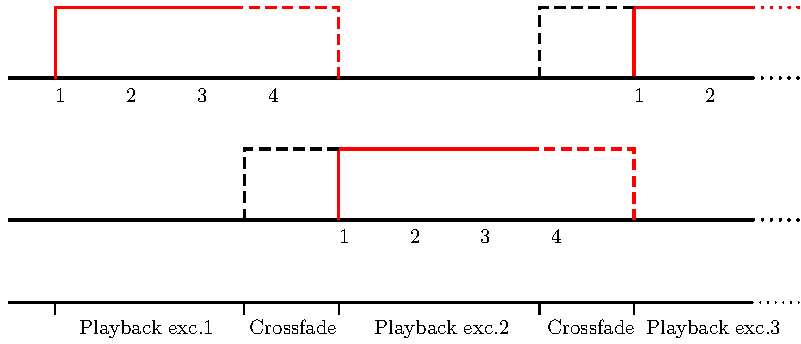
\includegraphics[scale=1]{Figures/crossfade.pdf}
    \rule{27em}{0.5pt}
  \caption[Audio crossfade]{Handling of audio crossfades. The red rectangles indicated the content of the excerpt, and dashed lines indicate crossfades. Note that the playback involves more than just the excerpts' content: we use the portion of audio before it during the fade-in to achieve a beat-level synchronization. The indices indicate the number of the beats inside the excerpts.}
  \label{fig:crossfade}
\end{center}
\end{figure}
\\The audio of the global pipeline is collected by the TCP sink, that is in charge of streaming this content over the TCP port 8070. This stream will be collected by the client application.


%%%%%%%%%%%%%%%%%%%%%%%%%%%%%%%%%%%%%%%%%%%%%%%%%%%%%%%%%%%%%%%%%%%%%%%%%%%%%%%%%%%%%%%%%%%%%%%%%%%%%%%%%%%%%%%%%%%%%%%%%%%%%%%%%%%%%%%%%%%%%%%%%%%%%%%%%%%%%%%%%%%%%%%%%%%%%%%%%%%%%%%%%%%%%%%%%%%%%%%%%%%%%%%
%%%%%%%%%%%%%%%%%%%%%%%%%%%%%%%%%%%%%%%%%%%%%%%%%%%%%%%%%%%%%%%%%%%%%%%%%%%%%%%%%%%%%%%%%%%%%%%%%%%%%%%%%%%%%%%%%%%%%%%%%%%%%%%%%%%%%%%%%%%%%%%%%%%%%%%%%%%%%%%%%%%%%%%%%%%%%%%%%%%%%%%%%%%%%%%%%%%%%%%%%%%%%%%
%%%%%%%%%%%%%%%%%%%%%%%%%%%%%%%%%%%%%%%%%%%%%%%%%%%%%%%%%%%%%%%%%%%%%%%%%%%%%%%%%%%%%%%%%%%%%%%%%%%%%%%%%%%%%%%%%%%%%%%%%%%%%%%%%%%%%%%%%%%%%%%%%%%%%%%%%%%%%%%%%%%%%%%%%%%%%%%%%%%%%%%%%%%%%%%%%%%%%%%%%%%%%%%
%%%%%%%%%%%%%%%%%%%%%%%%%%%%%%%%%%%%%%%%%%%%%%%%%%%%%%%%%%%%%%%%%%%%%%%%%%%%%%%%%%%%%%%%%%%%%%%%%%%%%%%%%%%%%%%%%%%%%%%%%%%%%%%%%%%%%%%%%%%%%%%%%%%%%%%%%%%%%%%%%%%%%%%%%%%%%%%%%%%%%%%%%%%%%%%%%%%%%%%%%%%%%%%

\section{The client application}
\label{sec:rtclient}
The client application consists of a web-application hosted by the Flask application running on the server. To access it, the client needs to connect to the address \texttt{http://server\_address:5000} on a browser. We entirely designed the graphical user interface of this application with the software \textit{Adobe Photoshop CS6\footnote{\url{http://www.adobe.com/products/photoshop.html}}}, with the intention of providing a ``metallic'' looking (that could resemble of the analogue synthesizers used in early Phonos records) coupled with the presence of elements (sliders and knob controllers) whose purpose could be easily understood by users. This interface is shown in Figure~\ref{fig:gui1}.

\begin{figure}[h]
\hskip -0.8cm
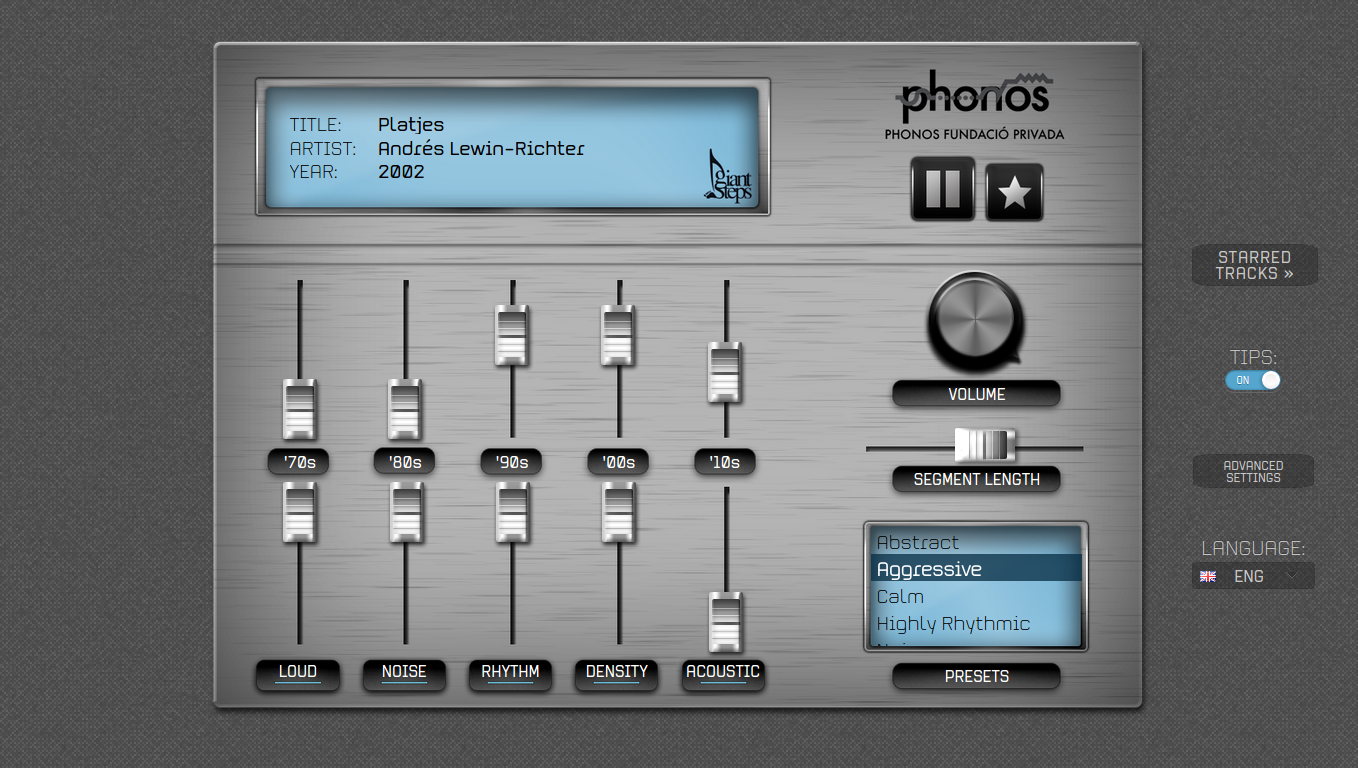
\includegraphics[scale=0.34]{Figures/gui1.png}
    \rule{27em}{0.5pt}
  \caption[Client application user interface]{Client application GUI.}
  \label{fig:gui1}

\end{figure}

This interface provides several ways for the user to control the music flow. Each time the user interacts with one of them, an HTTP post request is done from the client machine to the server, resulting in a change of the candidates for the playlist. \\
There are ten sliders: five of them are related to the year of release of the musical pieces, the other five are instead related to intrinsic characteristics of the music. In this way, the user has control both over the decade, and both over the type of music he wants to listen to. The motivation of this design choice is that we want to make the process of discovering music interactive while preserving ease of use. Furthermore, the suddivision of music into decades may be particularly useful in the use at the exhibition, since visitors could be particularly interested in hearing the differences between the works belonging to just a particular era over the entire 40 years life of Phonos. \\The five sliders for music features are:
\begin{itemize}
\item Loudness
\item Noisiness: related to the dissonance of the signal
\item Rhythm: higher values of the slider lead to excerpts with a high amount of onsets on high frequencies
\item Density: higher values of the slider lead to excerpts where many Barkbands have a considerable amount of energy
\item Acousticness: sets the ratio Acoustic/Electronic. Lower values of the slider mostly lead to purely electronic music.
\end{itemize}
The ranges of the internally managed sliders' values are dinamically generated during the computation of the FastMap: once the corresponding values for all the excerpts have been collected, these are sorted and we then pick the minimum, the maximum, and the first, second and third quartile for the values related to each descriptors. Therefore keeping the slider of the loudness at maximum will for instance lead to all the excerpts whose loudness value is between the third quartile and the maximum value of loudness of all excerpts. Step values for these five descriptors are calculated after the computation of the FastMap and kept in a separate JSON file. \\
The GUI additionally provides a set of presets for the values of these five sliders, a monitor for displaying information about the currently playing track, a slider for selecting the length of the audible segments (from 1 to 5 bars), and a knob for the volume (which controls the volume element of the global pipeline explained in Table~\ref{table:pipeline}). \\ By clicking on the button with a star on it, the user has the possibility of marking a track as favorite. The list of \textit{``starred tracks''} is accessible on the second page of the GUI (shown in Figure~\ref{fig:gui2}), together with the list of the five last played track. The motivation behind this choice is to give the user the chance to keep track of the songs he has been finding interesting. At the exhibition, visitors may be particularly interesting in looking for more information about a track they like. \\ 
Furthermore, this interface is offered in three different languages: English, Spanish and Catalan. This has been done to increase the usability of the software at the exhibition, taking into account possible cultural differences. \\
The interface fully supports touch screen environments and is based on HTML5, CSS3 and Javascript. Many features of the jQuery library for Javascript are also used. The range sliders are based on \textit{noUiSlider\footnote{\url{http://refreshless.com/nouislider/}}}, while the volume knob is based on \textit{jQuery Knob\footnote{\url{http://anthonyterrien.com/knob/}}}. The design of the graphical user interface has been directed toward the ease of use, for the visitors of the Museum may not be particularly confortable with the use of software or of tools related to music manipulation or playback. \\
Corcerning the reception of the audio streaming, many efforts have been done in order to achieve low-latency in the transmission of the multimedia content. Specifically, tries have involved the use of an icecast\footnote{\url{http://icecast.org/}} server or specific GStreamer units to try to implement low-latency audio streaming directly accessible from the html5 page. None of these tries have fully worked: latency was always registered around 5 seconds, probably due to browser's buffering techiques. This performance was clearly unacceptable. Thus we decided to exploit the functionalities provided by VideoLAN VLC\footnote{\url{http://www.videolan.org/vlc/index.html}}: specifically, we wrote a daemon for the interactive kiosk that launches a hidden instance of VLC as soon as it detects a stream on the TCP port 8070 (generated by the TCPSink of GStreamer). This istance of VLC is then in charge of capturing and playing this stream of multimedia content. The main advantages of this choice are:
\begin{itemize}
\item Good latency (around 500ms)
\item The user is completely unaware of this, for it is possible to start VLC in a daemon mode, thus without any sort of windows popping up. 
\end{itemize}
Generally, for real-time web application, the use of web protocols RTP (Real Time Protocol) and RTSP (Real Time Streaming Protocol) is suggested, as this usually allows low latencies in multimedia streaming. The use of these protocols for this application have not been taken into account, for their use requires to be integrated into Adobe Flash\footnote{\url{http://get.adobe.com/it/flashplayer/}} applications, which are generally discouraged as they introduce additional constraints and are usually not supported on touch devices. Furthermore, we had no experience with this particular programming language, and it could have not been feasible to develop the audio streaming in this language before the inauguration of the exhibition.

\begin{figure}[h]
\hskip -0.4cm
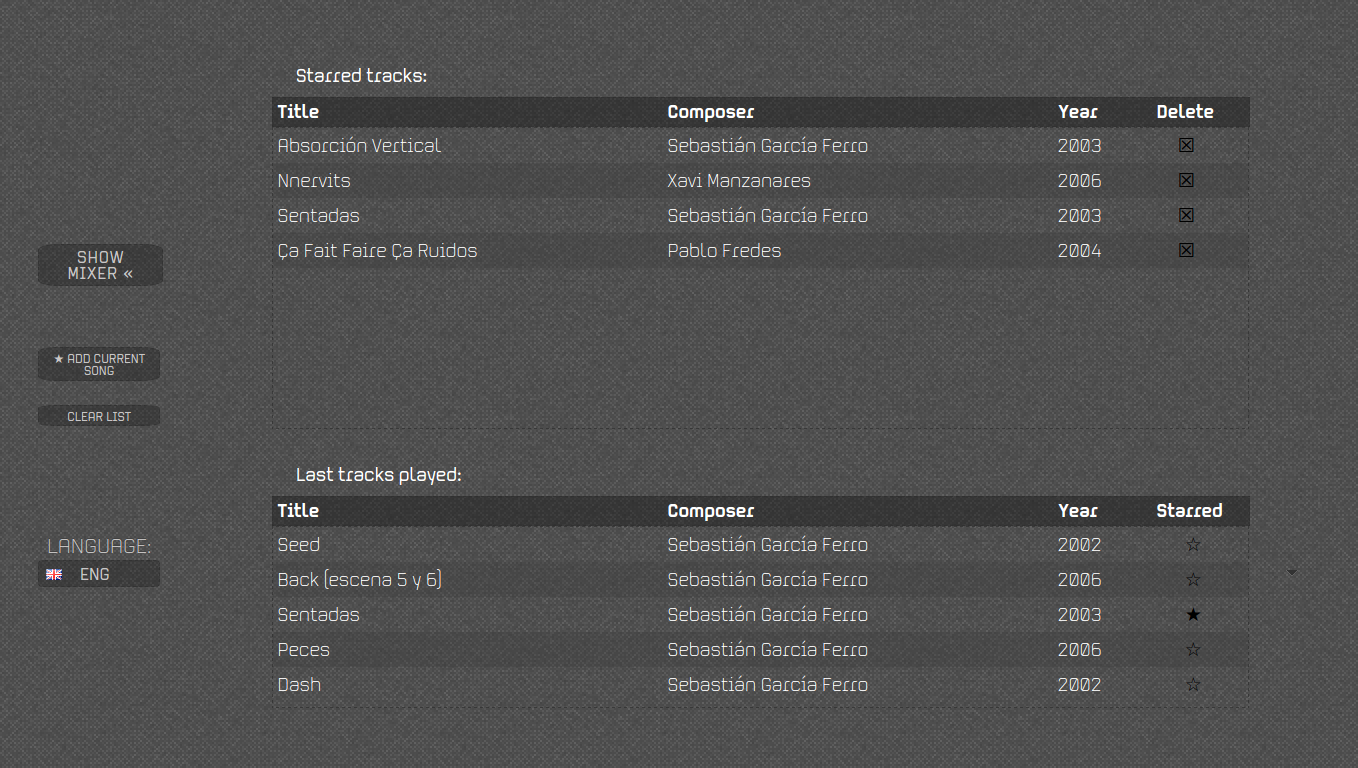
\includegraphics[scale=0.32]{Figures/gui2.png}
    \rule{27em}{0.5pt}
  \caption[The second page of the user interface]{The second page of the client application GUI, providing information about favorite and last played tracks.}
  \label{fig:gui2}
\end{figure}

The performance of this real-time system will be analyzed in the following chapter.